\documentclass[10pt,a4paper]{article}	%字体、纸张
\usepackage{xeCJK}	%中文
\usepackage[a4paper,left=20mm,right=20mm,top=25mm,bottom=20mm]{geometry}	%页边距
\usepackage{fancyhdr}	%页眉、页脚
\usepackage{indentfirst}	%首行缩进
\usepackage{graphicx}	%图片
\usepackage{textcomp}
\usepackage{subfigure}	
\usepackage{enumitem}
\usepackage{tabularx}
\usepackage{multirow}
\usepackage{caption}
\usepackage{amsmath}	%公式对齐
\usepackage{tikz-feynman}

\newcommand{\nexp}{光电效应测普朗克常数}

%————页眉、页脚设置————
\thispagestyle{plain}
\pagestyle{fancy}
\fancyhf{}
\fancyhead[R]{PB22000195 王元叙}
\fancyhead[L]{\nexp}	%————————————
\fancyfoot[C]{\thepage}
\renewcommand{\headrulewidth}{0pt}
\renewcommand{\footrulewidth}{0pt}
%————————————

\setenumerate[1]{itemsep=0pt,partopsep=0pt,parsep=\parskip,topsep=5pt}
\setlength{\parindent}{2em}
\renewcommand\arraystretch{1.3}

\makeatletter
\newenvironment{figurehere}
{\def\@captype{figure}}
{}
\newenvironment{tablehere}
{\def\@captype{table}}
{}
\makeatother

\begin{document}
	%————起始————
	\vspace*{-5em}
	\begin{center}
		\includegraphics[width=0.6\textwidth]{Picture//USTC}\\
		\Large \textbf{大学物理-基础实验|数据分析}\\[5mm]

		\normalsize
		\begin{tabular}{ll}
			姓名 & \textbf{王元叙}\\
			学号 & \textbf{PB22000195}\\
			班级 & \textbf{22级少年班学院5班}\\
			日期 & \textbf{2023年5月10日}\\	
		\end{tabular}\\[5mm]

		\LARGE \textbf{\nexp}\\[5mm]	

	\end{center}
	%————————————

	\section{基础实验数据分析}

	\subsection{零电流法测量普朗克常数}

	\begin{tablehere}
		\caption*{\bf 表1 零电流法测原始数据}
		\noindent
		\begin{center}
			\newcolumntype{Y}{>{\centering\arraybackslash}X}
			\begin{tabularx}{0.95\linewidth}{|c|Y|Y|Y|Y|Y|}
				\hline
				波长/nm    & 577   & 546   & 436   & 45    & 365 \\ \hline
				频率/$10^{14}$Hz & 5.199 & 5.495 & 6.880 & 7.407 & 8.219 \\ \hline
				遏止电压/V & 0.488 & 0.594 & 1.152 & 1.466 & 1.738 \\ \hline
				\end{tabularx}
		\end{center}
		\vspace*{1em}
	\end{tablehere}

	\begin{figurehere}
		\centering
		\includegraphics[width=.95\linewidth]{pics/1.png}
		\caption*{\bf 图1: 零电流法最小二乘法拟合}
	\end{figurehere}


	拟合得到直线方程中,曲线斜率、截距分别为为
	$$
	k=0.421\times 10^{-14}, b = -1.708 \times 10^{-14}
	$$
	
	计算得到普朗克常数
	$$
	\begin{aligned}
		h&=e \frac{U_0}{f} = ek \\
		&=1.602 \times 10 ^ {-19} \times 0.421 \times 10^{-14} \, \text{J$\, \cdot $s}\\
		&=6.736\times 10^{-34}\, \text{J$\, \cdot $s} \\
	\end{aligned}
	$$

	对比普朗克常数标准值 $h_0 = 6.63\times 10^{-34}\, \text{J$\, \cdot $s}$ ,相对误差为
	\[
		h_{\text{相对误差}}=\dfrac{|h-h_0|}{h_0}=\dfrac{6.736-6.63}{6.63}=1.60\% 
	\]

	得到红限频率为
	\[
		\begin{aligned}
			\nu &= \frac{1.708}{0.421} \times 10^{-14} \mathrm{~Hz}\\
			&= 4.057 \times 10^{-14}  \mathrm{~Hz}\\
		\end{aligned}
	\]

	溢出功
	\[
		\begin{aligned}
			A &= 1.602 \times 10 ^ {-19} \times 1.708 \times 10^{-14} \, \text{J$\, \cdot $s}\\
			&=2.736\times 10^{-39}\mathrm{~J} \\
		\end{aligned}
	\]
	
	\subsection{补偿法测量普朗克常数}

	\begin{tablehere}
		\caption*{\bf 表2 补偿法测原始数据}
		\noindent
		\begin{center}
			\newcolumntype{Y}{>{\centering\arraybackslash}X}
			\begin{tabularx}{0.95\linewidth}{|c|Y|Y|Y|Y|Y|}
				\hline
				波长/nm    & 577   & 546   & 436   & 45    & 365 \\ \hline
				频率/$10^{14}$Hz & 5.199 & 5.495 & 6.880 & 7.407 & 8.219 \\ \hline
				遏止电压/V & 0.492 & 0.598 & 1.158 & 1.468 & 1.740 \\ \hline
				暗电流/$10^{-13}$A & -0.02 & -0.03 & -0.05 & -0.04 & -0.54 \\ \hline
				\end{tabularx}
		\end{center}
		\vspace*{1em}
	\end{tablehere}

	\begin{figurehere}
		\centering
		\includegraphics[width=.80\linewidth]{pics/2.png}
		\caption*{\bf 图2: 补偿法最小二乘法拟合}
	\end{figurehere}

	拟合得到直线方程中,曲线斜率、截距分别为为
	$$
	k=0.423\times 10^{-14}, b = -1.714 \times 10^{-14}
	$$
	
	计算得到普朗克常数
	$$
	\begin{aligned}
		h&=e \frac{U_0}{f} = ek \\
		&=1.602 \times 10 ^ {-19} \times 0.421 \times 10^{-14} \, \text{J$\, \cdot $s}\\
		&=6.776\times 10^{-34}\, \text{J$\, \cdot $s} \\
	\end{aligned}
	$$

	对比普朗克常数标准值 $h_0 = 6.63\times 10^{-34}\, \text{J$\, \cdot $s}$ ,相对误差为
	\[
		h_{\text{相对误差}}=\dfrac{|h-h_0|}{h_0}=\dfrac{6.776-6.63}{6.63}=2.21\% 
	\]

	得到红限频率为
	\[
		\begin{aligned}
			\nu &= \frac{1.714}{0.423} \times 10^{-14} \mathrm{~Hz}\\
			&= 4.071 \times 10^{-14}  \mathrm{~Hz}\\
		\end{aligned}
	\]

	溢出功
	\[
		\begin{aligned}
			A &= 1.602 \times 10 ^ {-19} \times 1.714 \times 10^{-14} \, \text{J$\, \cdot $s}\\
			&=2.748\times 10^{-39}\mathrm{~J} \\
		\end{aligned}
	\]

	\subsection{通过光阑孔径研究饱和光电流与光强的关系}

	取定入射距离为 $40 \mathrm{~cm}$

	\begin{tablehere}
		\caption*{\bf 表3 光阑孔径与饱和光电流关系}
		\noindent
		\begin{center}
			\newcolumntype{Y}{>{\centering\arraybackslash}X}
			\begin{tabularx}{0.95\linewidth}{|c|c|Y|Y|Y|Y|}
				\hline
				\multirow{2}[0]{*}{波长436/nm} & 光阑孔径$\Phi$/mm & 2 & 4 & 8 & 14.35\\ \cline{2-6}
					  & 饱和光电流$I_M$/$10^{-10}$A & 9.5 & 33.9 & 121.8 & 368 \\ \hline
				\multirow{2}[0]{*}{577/nm} & 光阑孔径$\Phi$/mm  & 2 & 4 & 8 & 14.35\\ \cline{2-6}
					  & 饱和光电流$I_M$/$10^{-10}$A & 1.1 & 3.7 & 13.6 & 40.7 \\ \hline
			\end{tabularx}
		\end{center}
		\vspace*{1em}
	\end{tablehere}

	由于光强 $P$ 正比于 $\Phi^2$ ,于是作图

	\begin{figurehere}
		\vspace*{1em}
		\centering
		\begin{minipage}[t]{0.5\textwidth}
		\centering
		\includegraphics[width=\linewidth]{pics/3.png}
		\caption*{\bf 图3.1 波长436nm}
		\end{minipage}
		\begin{minipage}[t]{0.5\textwidth}
		\centering
		\includegraphics[width=\linewidth]{pics/4.png}
		\caption*{\bf 图3.2 波长577nm}
		\end{minipage}
	\end{figurehere}

	两条图线分别指出:
	$$
	\begin{aligned}
		I_{M,436}= 1.76 \Phi^2 + 7.98 \\
		I_{M,577}= 0.19 \Phi^2 + 0.61
	\end{aligned}
	$$

	从中可以看出,饱和光电压 $I$ 与光强 $P$ 成线性关系,并且截距均在实验误差允许范围内。因此我们可以近似认为,饱和光电压 $I$ 正比于光强 $P$ 。

	\subsection{通过入射距离研究饱和光电流与光强的关系}

	取定光阑孔径为 $2 \mathrm{~mm}$

	\begin{tablehere}
		\caption*{\bf 表4 入射距离与饱和光电流关系}
		\noindent
		\begin{center}
			\newcolumntype{Y}{>{\centering\arraybackslash}X}
			\begin{tabularx}{0.95\linewidth}{|c|c|Y|Y|Y|Y|Y|Y|}
				\hline
				\multirow{2}[0]{*}{波长436/nm} & 入射距离L/cm & 30 & 32 & 34 & 36 & 38 & 40\\ \cline{2-8}
					  & 饱和光电流$I_M$/$10^{-10}$A & 20.9 & 16.2 & 14.8 & 12.3 & 10.4 & 9.0 \\ \hline
				\multirow{2}[0]{*}{577/nm} & 入射距离LL/cm   & 30 & 32 & 34 & 36 & 38 & 40 \\ \cline{2-8}
					  & 饱和光电流$I_M$/$10^{-10}$A & 2.27 & 1.91 & 1.60 & 1.31 & 1.20 & 1.07 \\ \hline
			\end{tabularx}
		\end{center}
		\vspace*{1em}
	\end{tablehere}

	
	由于光强 $P$ 正比于 $L^{-2}$ ,于是作图

	\begin{figurehere}
		\vspace*{1em}
		\centering
		\begin{minipage}[t]{0.5\textwidth}
		\centering
		\includegraphics[width=\linewidth]{pics/5.png}
		\caption*{\bf 图4.1 波长436nm}
		\end{minipage}
		\begin{minipage}[t]{0.5\textwidth}
		\centering
		\includegraphics[width=\linewidth]{pics/6.png}
		\caption*{\bf 图4.2 波长577nm}
		\end{minipage}
	\end{figurehere}

	两条图线分别指出
	$$
	\begin{aligned}
		I_{M,436}= 2.37 L^{-2} - 5.94 \\
		I_{M,577}= 0.25 L^{-2} - 0.51
	\end{aligned}
	$$

	从中可以看出,饱和光电压 $I$ 与光强 $P$ 成线性关系,并且截距均在实验误差允许范围内。因此我们可以近似认为,饱和光电压 $I$ 正比于光强 $P$ 。
	\newpage
	
	\section{进阶实验}

	使用拐点法测量了四种波长单色光的遏止电压,原始数据见附录(在 $\lambda = 362\mathrm{~nm}$ 的数据当中,虽然原始数据记录了101组,但是这里只对前61组绘图,因为后面的数据中电流已经大于0,对拐点法无用)

	\begin{figurehere}
		\centering
		\includegraphics[width=.80\linewidth]{pics/7.png}
		\caption*{\bf 图5.1: 波长365m,电压区间-1900~-1660 mV}
	\end{figurehere}

	拐点位于 $-1780\mathrm{~mV}$ 的位置。

	\begin{figurehere}
		\centering
		\includegraphics[width=.80\linewidth]{pics/8.png}
		\caption*{\bf 图5.2: 波长405nm,电压区间-1600~-1400 mV}
	\end{figurehere}

	拐点位于 $-1528\mathrm{~mV}$ 的位置。

	\begin{figurehere}
		\centering
		\includegraphics[width=.80\linewidth]{pics/9.png}
		\caption*{\bf 图5.3: 波长436nm,电压区间-1250~-1050 mV}
	\end{figurehere}

	拐点位于 $-1198\mathrm{~mV}$ 的位置。

	\begin{figurehere}
		\centering
		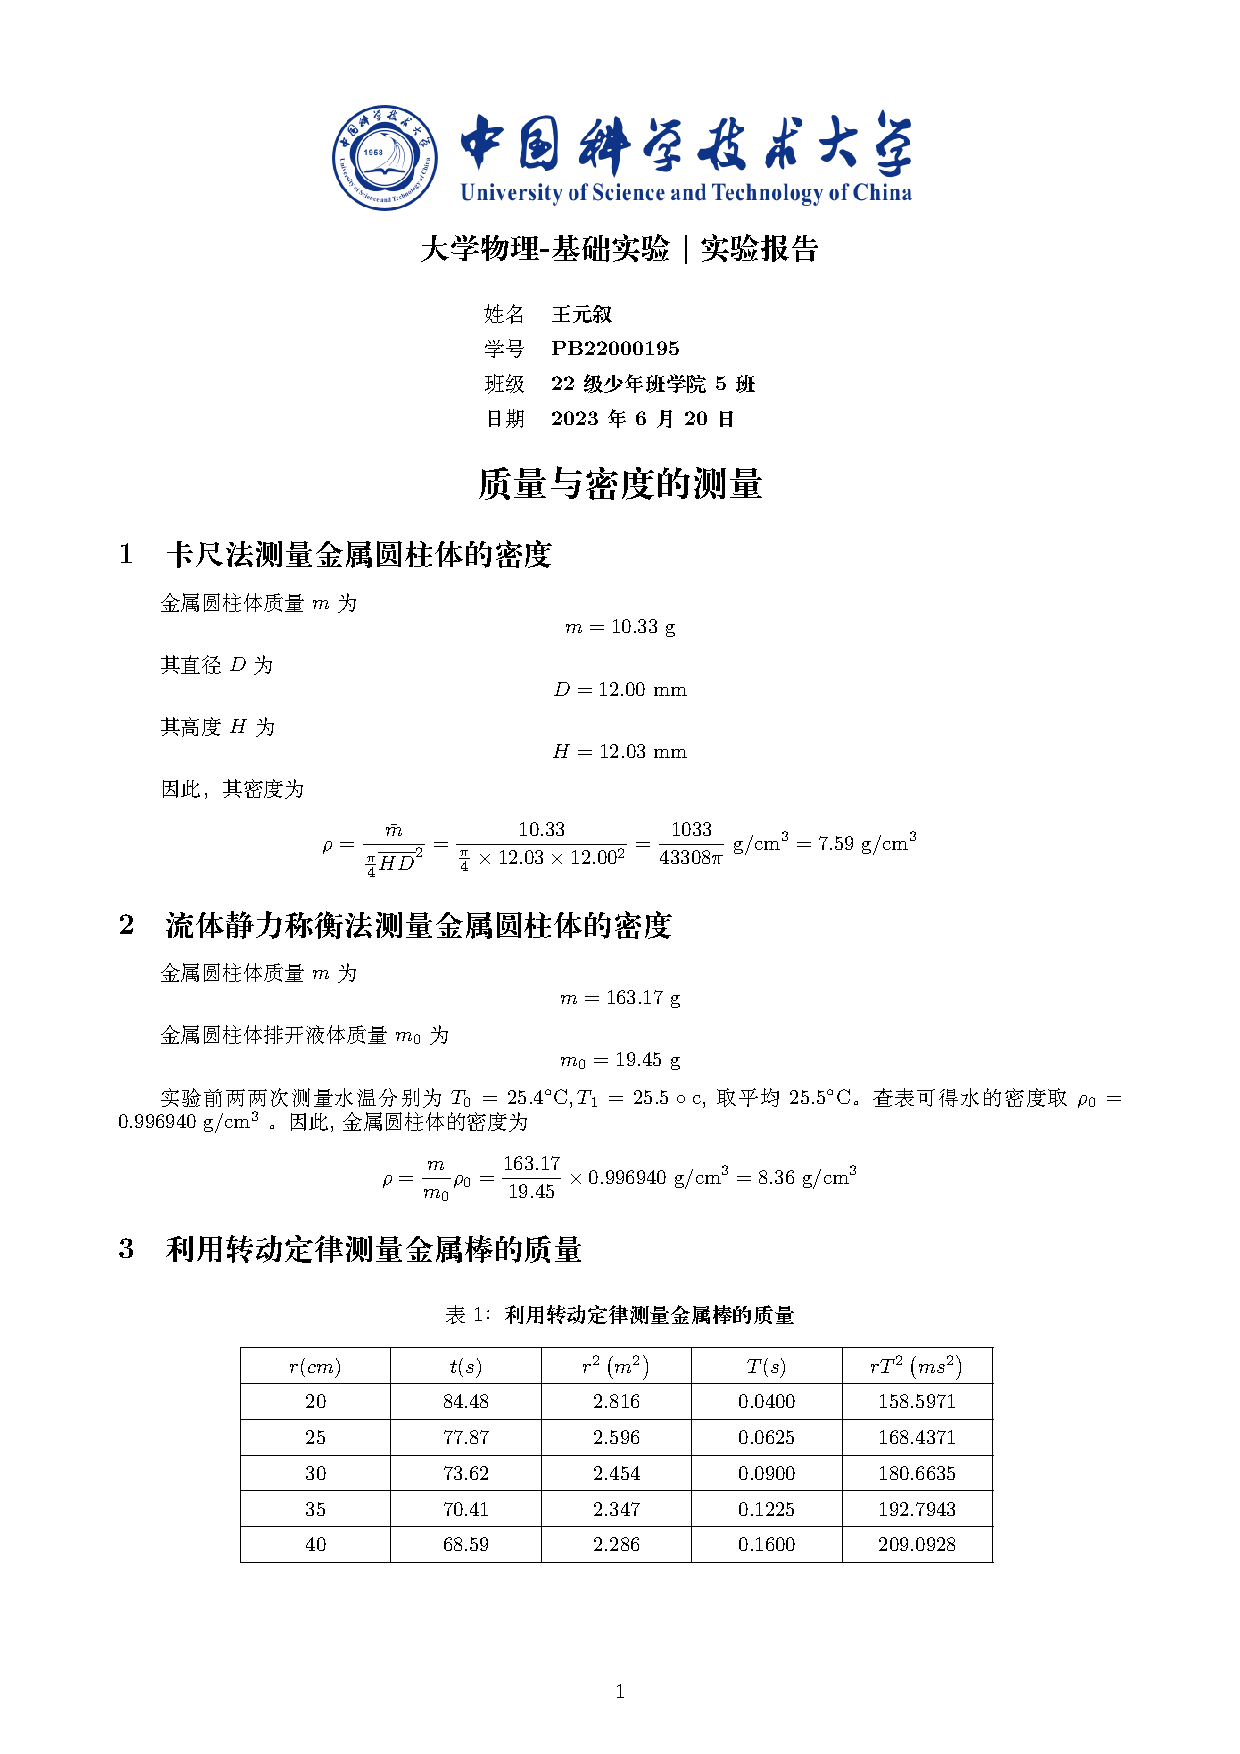
\includegraphics[width=.80\linewidth]{pics/10.png}
		\caption*{\bf 图5.4: 波长546nm,电压区间-700~-500 mV}
	\end{figurehere}

	拐点位于 $-632\mathrm{~mV}$ 的位置。

	\newpage

	\begin{tablehere}
		\caption*{\bf 表5 拐点法测原始数据}
		\noindent
		\begin{center}
			\newcolumntype{Y}{>{\centering\arraybackslash}X}
			\begin{tabularx}{0.95\linewidth}{|c|Y|Y|Y|Y|}
				\hline
				波长/nm      & 546   & 436   & 45    & 365 \\ \hline
				频率/$10^{14}$Hz  & 5.495 & 6.880 & 7.407 & 8.219 \\ \hline
				遏止电压/V & 0.632 & 1.198 & 1.528 & 1.780 \\ \hline
				\end{tabularx}
		\end{center}
		\vspace*{1em}
	\end{tablehere}

	\begin{figurehere}
		\centering
		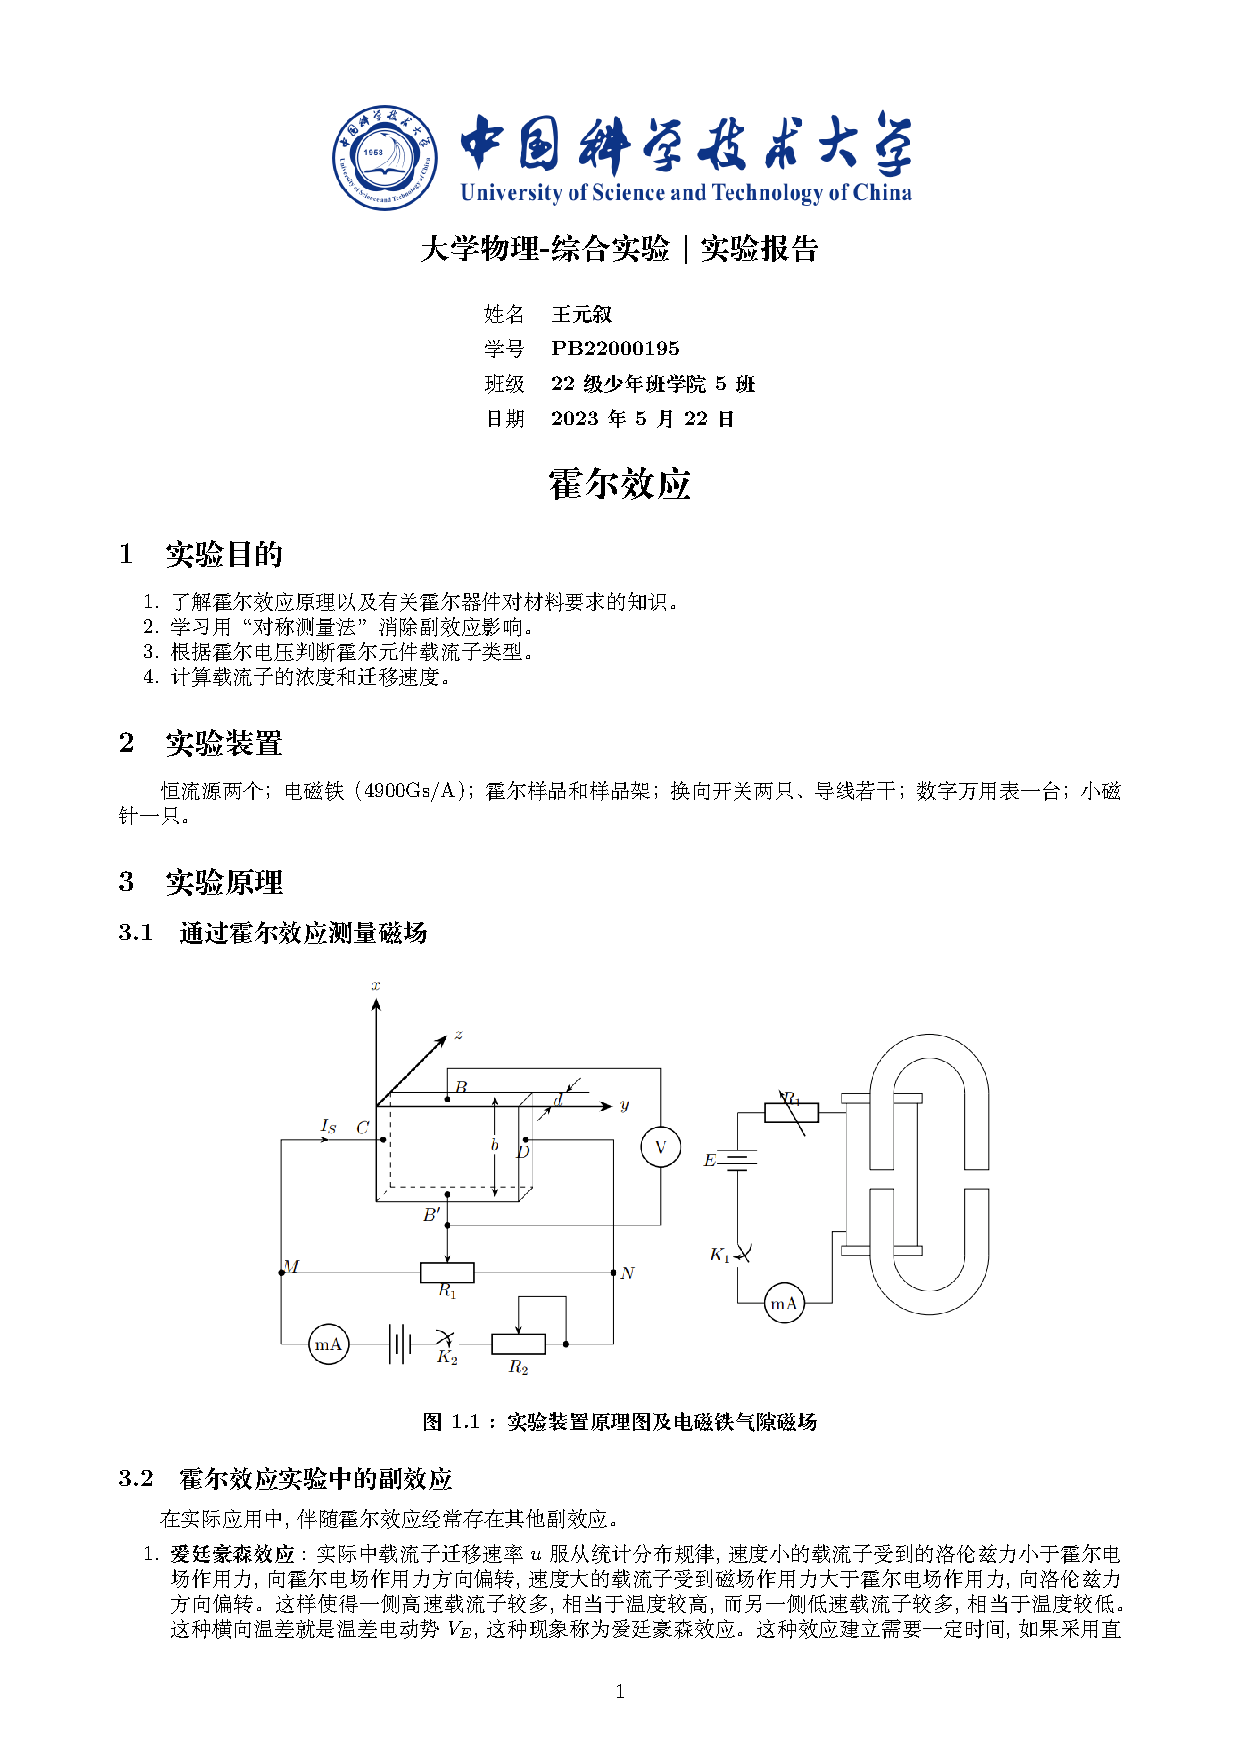
\includegraphics[width=.80\linewidth]{pics/11.png}
		\caption*{\bf 图6: 拐点法法最小二乘法拟合}
	\end{figurehere}

	拟合得到直线方程中,曲线斜率为
	$$
	k=0.431\times 10^{-14}
	$$
	
	计算得到普朗克常数
	$$
	\begin{aligned}
		h&=e \frac{U_0}{f} = ek \\
		&=1.602 \times 10 ^ {-19} \times 0.431 \times 10^{-14} \, \text{J$\, \cdot $s}\\
		&=6.909\times 10^{-34}\, \text{J$\, \cdot $s} \\
	\end{aligned}
	$$

	对比普朗克常数标准值 $h_0 = 6.63\times 10^{-34}\, \text{J$\, \cdot $s}$ ,相对误差为
	\[
		h_{\text{相对误差}}=\dfrac{|h-h_0|}{h_0}=\dfrac{6.909-6.63}{6.63}=4.21\% 
	\]
	
	\section{误差分析}

	在使用三种方法测量遏止电压进而测量普朗克常数的过程当中,理论上来看,零电流法的误差应当大于补偿法的误差,补偿法的误差应当大于拐点法的误差。然而在实际实验中,后两种方法得到的误差都相对较大,原因可能有以下几点:
	\begin{enumerate}
		\item 补偿法测量普朗克常数,由于暗电流长时间不稳定,因此读数误差较大,造成最终测量结果误差增大
		\item 在使用补偿法测量的过程中,实际实验的得到的图像并不存在清晰的拐点,曲线的斜率逐渐增大,很难判断拐点的正确位置,造成了较大的实验误差。
		\item 补偿法测量中,自动扫描得到的数据有些许误差,增大了判断拐点的难度
	\end{enumerate}

	%————正文————
\end{document}
